\documentclass[10pt,a4paper]{article}
\usepackage[T1]{fontenc}
\usepackage{amsmath}
\usepackage{amsfonts}
\usepackage{amssymb}
\usepackage{graphicx}
\usepackage{enumitem}
\usepackage{titlesec}
\usepackage{geometry}
\geometry{a4paper, margin=1in}
\usepackage{hyperref} 
\usepackage[portuguese]{babel}

% Configurações de títulos para um visual mais limpo e profissional
\titleformat{\section}[block]{\bfseries\Large\raggedright}{}{0em}{}
\titlespacing{\section}{0pt}{1.5em}{1em}

\title{Plano de Formação: Linux - Serviços de Redes}
\author{Formador: [Seu Nome]}
\date{Data de Elaboração: [Data]}


\begin{document}
	
	\section*{Conteúdos}
	
	\subsection*{1. Serviços de rede}
	\vspace{-1.2em}
	\paragraph{}
	Nesta secção, vamos explorar como os serviços de rede são geridos no Linux, desde o seu início até ao encerramento, e os principais ficheiros e diretórios envolvidos neste processo.
	
	\begin{itemize}
		\item \textbf{Conceito Chave: O Papel do \texttt{systemd}} \\
		O **`systemd`** é o gestor de sistema e de serviços padrão na maioria das distribuições Linux modernas, substituindo sistemas mais antigos como o SysVinit. Ele usa "unidades" para gerir processos, o que lhe dá um controlo mais granular, robusto e eficiente sobre os serviços. Em vez de scripts de inicialização simples, as unidades `systemd` podem definir dependências, o que garante que os serviços iniciam na ordem correta.
		
		\item \textbf{Exemplo Detalhado: Análise do Estado de um Serviço} \\
		Vamos usar o comando `systemctl status` para obter informações detalhadas sobre o serviço de SSH (`sshd`). Uma imagem da saída deste comando pode ilustrar bem a informação disponível.
		
		\begin{figure}[h]
			\centering
			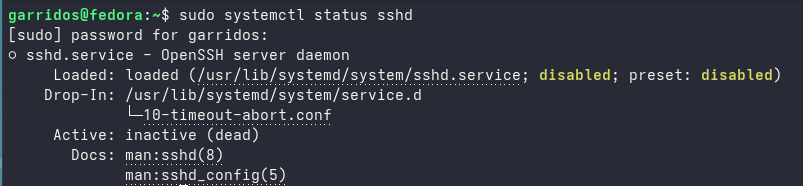
\includegraphics[width=0.8\textwidth]{img/systemctl_status.png}
			\caption{Exemplo da saída do comando \texttt{systemctl status sshd}. \textit{Fonte: garridos.}}
			\label{fig:systemctl_status}
		\end{figure}
		
		A resposta mostra o estado atual do serviço (ativo/inativo), o PID (Process ID), há quanto tempo está a correr e as últimas linhas dos seus logs. Isto é crucial para diagnosticar rapidamente se um serviço está a funcionar.
		
		\item \textbf{Dicas de Resolução de Problemas}
		\begin{itemize}
			\item **Verificação de Logs**: Se um serviço não inicia, o primeiro passo é verificar os seus logs. O comando `journalctl -u [serviço]` mostra todo o histórico de logs do serviço, o que pode revelar a causa do erro.
			\item **Estado de Ativação**: Use `systemctl is-enabled [serviço]` para verificar se um serviço está configurado para iniciar automaticamente no arranque do sistema.
		\end{itemize}
		
		\item \textbf{Exercício de Consolidação}
		1. Inicie e verifique o estado do serviço web Apache (`httpd`).
		2. Habilite o Apache para iniciar automaticamente no próximo arranque do sistema.
		
		\item \textbf{Para Aprofundar}
		Explore a diferença entre os comandos `systemctl start`, `restart` e `reload`. Investigar a estrutura de um ficheiro de unidade `.service` em `/etc/systemd/system/` também é um excelente próximo passo.
	\end{itemize}
	
	---
	
	\subsection*{2. XINET.d}
	\vspace{-1.2em}
	\paragraph{}
	O \texttt{xinetd} (e o seu antecessor, o \texttt{inetd}) funciona como um "super-servidor" que gere a inicialização de serviços de rede que não precisam de estar ativos a todo o momento, como o \texttt{telnet} ou \texttt{ftp}. Ele espera por pedidos de conexão numa porta específica e, quando um pedido chega, inicia o serviço correspondente.
	
	\begin{itemize}
		\item \textbf{Conceito Chave: Servidor "On-Demand"} \\
		O \texttt{xinetd} economiza recursos do sistema, pois os serviços geridos por ele só correm quando necessário, em vez de estarem sempre ativos.
		
		\item \textbf{Exemplo Detalhado: Configuração de um Serviço} \\
		Vamos analisar o ficheiro de configuração do serviço \texttt{telnet} em \texttt{/etc/xinet.d/telnet}.
		\begin{verbatim}
			service telnet
			{
				disable         = yes
				id              = telnet-ipv4
				type            = UNLISTED
				...
			}
		\end{verbatim}
		A linha \texttt{disable = yes} é a chave: para ativar o serviço, deve ser alterada para \texttt{no}.
		
		\item \textbf{Dicas de Resolução de Problemas} \\
		\begin{itemize}
			\item Se um serviço gerido por \texttt{xinetd} não funciona, verifique o ficheiro de configuração correspondente em \texttt{/etc/xinet.d/} para ter a certeza de que a opção \texttt{disable} está definida como \texttt{no}.
		\end{itemize}
		
		\item \textbf{Exercício de Consolidação} \\
		1. Encontre o ficheiro de configuração do serviço \texttt{ftp} no diretório \texttt{/etc/xinet.d/}.
		2. Altere o valor da opção \texttt{disable} para habilitá-lo.
		3. Reinicie o serviço \texttt{xinetd} para que as alterações entrem em vigor.
	\end{itemize}
	
	---
	
	\subsection*{3. TCPWrappers}
	\vspace{-1.2em}
	\paragraph{}
	O \texttt{TCPWrappers} é uma ferramenta de segurança simples mas eficaz para controlar o acesso a serviços de rede, atuando como um "firewall de nível de serviço". Ele permite a criação de regras de acesso (permitir/negar) baseadas em endereços IP ou nomes de host.
	
	\begin{itemize}
		\item \textbf{Conceito Chave: O Ciclo \texttt{hosts.allow} -> \texttt{hosts.deny}} \\
		As regras são processadas numa ordem específica: o sistema verifica primeiro o ficheiro \texttt{/etc/hosts.allow}. Se uma regra corresponder, o acesso é concedido e o \texttt{hosts.deny} é ignorado. Se não houver correspondência, o sistema verifica o \texttt{hosts.deny}. Se uma regra corresponder, o acesso é negado.
		
		\item \textbf{Exemplo Detalhado: Regras de Acesso} \\
		\begin{verbatim}
			Em /etc/hosts.allow:
			sshd: 192.168.1.100
			
			Em /etc/hosts.deny:
			sshd: ALL
		\end{verbatim}
		Neste exemplo, apenas a máquina com o IP \texttt{192.168.1.100} pode aceder ao serviço SSH. Todos os outros são bloqueados pela regra em \texttt{hosts.deny}.
		
		\item \textbf{Dicas de Resolução de Problemas} \\
		\begin{itemize}
			\item Cuidado com a ordem das regras! Uma regra ampla em \texttt{hosts.allow} pode anular regras mais específicas em \texttt{hosts.deny}.
		\end{itemize}
		
		\item \textbf{Exercício de Consolidação} \\
		1. Adicione uma regra para permitir o acesso ao serviço \texttt{ftp} a partir de um IP específico.
		2. Adicione uma segunda regra para negar o acesso a \texttt{ftp} a todos os outros IPs, exceto ao endereço do passo 1.
	\end{itemize}
	
	---
	
	\subsection*{4. NIS}
	\vspace{-1.2em}
	\paragraph{}
	O NIS (Network Information Service) é um sistema de diretório centralizado que permite que informações de contas de utilizadores, grupos e hosts sejam distribuídas por uma rede. É útil para ambientes de rede pequenos e uniformes.
	
	\begin{itemize}
		\item \textbf{Conceito Chave: Autenticação Centralizada} \\
		O NIS permite que um utilizador inicie sessão em qualquer máquina cliente na rede com as mesmas credenciais, pois as informações da conta são geridas num servidor central (o servidor NIS).
		
		\item \textbf{Exemplo Detalhado: Listar Utilizadores NIS} \\
		Após a configuração do cliente, podemos listar os utilizadores do servidor NIS com o comando \texttt{ypcat}.
		\begin{verbatim}
			$ ypcat passwd
		\end{verbatim}
		Este comando mostra o conteúdo do mapa \texttt{passwd} do NIS, que é uma lista dos utilizadores e suas informações.
		
		\item \textbf{Exercício de Consolidação} \\
		1. Use o comando \texttt{ypwhich} para verificar a que servidor NIS a sua máquina cliente está conectada.
		2. Use o comando \texttt{ypcat} para listar as contas de grupo disponíveis.
	\end{itemize}
	
	---
	
	\subsection*{5. DHCP}
	\vspace{-1.2em}
	\paragraph{}
	O DHCP (Dynamic Host Configuration Protocol) é o protocolo padrão para atribuir configurações de rede (como endereços IP) a dispositivos de forma automática.
	
	\begin{itemize}
		\item \textbf{Conceito Chave: O Processo DORA} \\
		O DHCP funciona através de um processo de quatro etapas: **D**iscover (descoberta), **O**ffer (oferta), **R**equest (pedido) e **A**cknowledge (confirmação). Uma imagem pode ilustrar bem este fluxo.
		
		\begin{figure}[h]
			\centering
			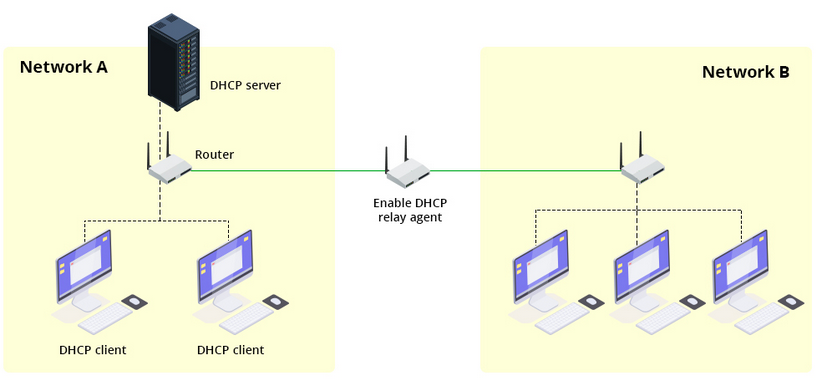
\includegraphics[width=0.8\textwidth]{img/dhcp_dora.png}
			\caption{Diagrama do processo DORA (Discover, Offer, Request, Acknowledge). \textit{Fonte: https://www.manageengine.com/products/oputils/images/network-a-b.jpg.}}
			\label{fig:dhcp_dora}
		\end{figure}
		
		\item \textbf{Exemplo Detalhado: Configuração de uma Sub-rede} \\
		Um exemplo de uma configuração no ficheiro \texttt{/etc/dhcp/dhcpd.conf} para a sub-rede \texttt{192.168.1.0/24}:
		\begin{verbatim}
			subnet 192.168.1.0 netmask 255.255.255.0 {
				range 192.168.1.100 192.168.1.200;
				option routers 192.168.1.1;
				option domain-name-servers 8.8.8.8, 8.8.4.4;
				default-lease-time 600;
				max-lease-time 7200;
			}
		\end{verbatim}
		
		\item \textbf{Dicas de Resolução de Problemas} \\
		\begin{itemize}
			\item Para IPs estáticos, use a diretiva \texttt{host} para garantir que uma máquina específica receba sempre o mesmo IP.
			\item Se o cliente não recebe um IP, verifique os logs do servidor DHCP para ver se há erros de comunicação.
		\end{itemize}
		
		\item \textbf{Exercício de Consolidação} \\
		1. Crie uma entrada no seu ficheiro \texttt{dhcpd.conf} para atribuir um IP estático (por exemplo, \texttt{192.168.1.50}) a uma máquina específica, usando o seu endereço MAC.
		2. Após a alteração, reinicie o serviço DHCP.
	\end{itemize}
	
	---
	
	\subsection*{6. DNS}
	\vspace{-1.2em}
	\paragraph{}
	O DNS (Domain Name System) é a base da internet, atuando como um "livro de endereços" que traduz nomes de domínio em endereços IP.
	
	\begin{itemize}
		\item \textbf{Conceito Chave: Resolução de Nomes} \\
		Quando um utilizador digita um nome de domínio, o cliente DNS consulta o servidor DNS para obter o endereço IP correspondente, permitindo que a conexão seja estabelecida. Este processo é hierárquico, começando pelos servidores de raiz e descendo até ao servidor autoritativo para o domínio em questão. Uma imagem pode ilustrar bem esta hierarquia.
		
		\begin{figure}[h]
			\centering
			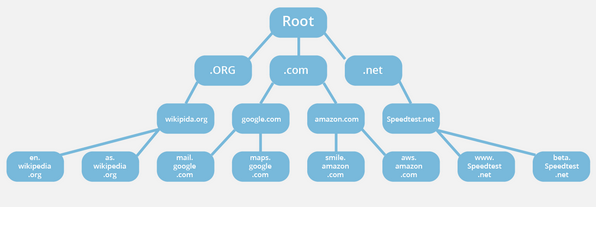
\includegraphics[width=0.8\textwidth]{img/dns_lookup.png}
			\caption{Fluxo de uma consulta DNS típica, mostrando a hierarquia de servidores. \textit{Fonte: https://www.cloudflare.com/img/learning/dns/glossary/dns-root-server/dns-root-server.png.}}
			\label{fig:dns_lookup}
		\end{figure}
		
		\item \textbf{Exemplo Detalhado: Ficheiro de Zona} \\
		Um ficheiro de zona simples para \texttt{exemplo.com}:
		\begin{verbatim}
			$TTL 86400
			@ IN SOA ns1.exemplo.com. admin.exemplo.com. (
			2023010101 ; Serial
			3600       ; Refresh
			1800       ; Retry
			604800     ; Expire
			86400      ; Minimum TTL
			)
			
			@   IN  NS  ns1.exemplo.com.
			@   IN  A   192.168.1.10
			
			www IN  A   192.168.1.11
			mail IN A   192.168.1.12
		\end{verbatim}
		
		\item \textbf{Dicas de Resolução de Problemas} \\
		\begin{itemize}
			\item Use `dig` ou `nslookup` para testar a resolução de nomes. Se o `dig` não funcionar, o problema pode estar na configuração do cliente ou do servidor.
		\end{itemize}
		
		\item \textbf{Exercício de Consolidação} \\
		1. No ficheiro de zona, adicione um novo registo \texttt{A} para um servidor de blog, com o nome \texttt{blog.exemplo.com} e o IP \texttt{192.168.1.20}.
		2. Recarregue o serviço DNS para aplicar as alterações.
	\end{itemize}
	
	---
	
	\subsection*{7. LOGS}
	\vspace{-1.2em}
	\paragraph{}
	Os logs são ficheiros de registo que fornecem informações sobre o que está a acontecer no sistema e nas aplicações. São cruciais para a monitorização e a resolução de problemas.
	
	\begin{itemize}
		\item \textbf{Conceito Chave: Onde Encontrar Informação} \\
		O diretório \texttt{/var/log} é o local central para a maioria dos logs do sistema e de aplicações. Cada ficheiro tem uma função específica (ex: \texttt{messages} para logs gerais, \texttt{auth.log} para autenticação).
		
		\item \textbf{Exemplo Detalhado: Analisar os Logs} \\
		Use \texttt{tail} para ver as últimas entradas de um ficheiro de log ou \texttt{grep} para procurar por mensagens específicas.
		\begin{verbatim}
			$ tail -f /var/log/messages
			$ grep "sshd" /var/log/auth.log
		\end{verbatim}
		
		\item \textbf{Exercício de Consolidação} \\
		1. Force um erro (por exemplo, ao tentar iniciar um serviço com a sintaxe incorreta).
		2. Use o comando \texttt{tail} ou \texttt{grep} para encontrar a mensagem de erro no ficheiro \texttt{/var/log/messages} e identifique o motivo do erro.
	\end{itemize}
	
\end{document}